\section{Results}
\label{game:results}
This section reports on the results after conducting the second experiment and analyzing the effects of the different game elements towards user engagement with Fastype. We also report on the playfulness of the game, feelings of competence, autonomy and relatedness in addition to testing and comparing the quality of annotations with the first experiment. In overall, these analysis will guide the rest of this research study towards answering the last research question regarding gamification and the corresponding hypothesis.

\subsection{Participants}
%Pre questionnaires 
%difference compared to first experiment 
It was mentioned in the previous section that the recruitment of participants has been done in a consistent way with the first experiment. The participation resulted in having 27 participants in total which is 3 participants less than the first experiment. Those who did not show up for the second experiment were either not at the university campus during the whole week of experiment or were sick and could not show up. However, among those 27 participants 11.1\% (namely 3 out of 27) of them were partcicipating for the first time. This small group of participants that were not part of the first user study were not presented with questions that involved comparisons or assessment of AnnotateMe with Fastype.

The pre-questionnaire for the second experiment was designed for gathering information about players' demographic data in addition to information related to their gameplay frequency. The questions related to gameplay frequency will provide approximate insights on how often participants play video games and see if this is a potential bias on the quality of annotations and evaluation of the game. Regarding demographic data (since 89\% of participants were participating for the second time) we report similar results: the average player is a 25 years old male student who studies in a computer science related field who occasionally plays video games with an average of 8 hours played during the last month. Figure \ref{fig:game-prequestionnaire} presents two graphs which report on the gamplay frequency (left figure) and average hours played (right figure) during last month. From the results of the pre-questionnaire, it can be concluded that our participants in general can not be considered as expert gamers based on their frequency of gameplay. However, on average the participants have a mix of different gaming frequency as observed on the left graph in Figure \ref{fig:game-prequestionnaire}. Therefore we argue that the population sample used for this experiment represents the potential average player of Fastype outside the experiment. 


\begin{figure}[]
    \centering
    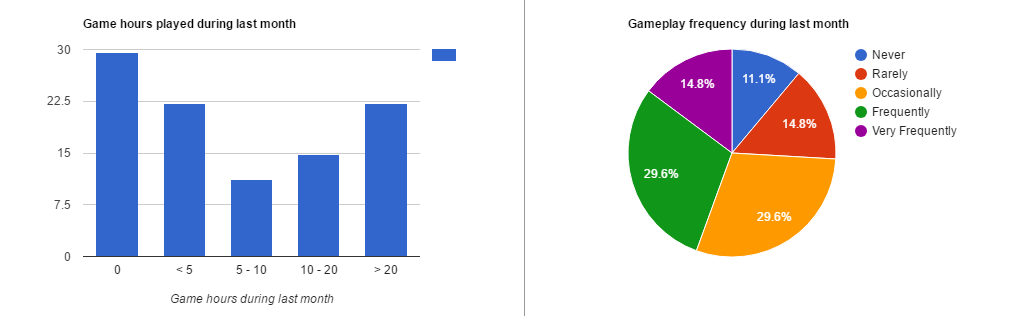
\includegraphics[width=\linewidth]{figures/experiment2/game-prequestionnaire.PNG}
    \caption{Results on participants' gameplay frequency for Experiment 2}
    \label{fig:game-prequestionnaire}
\end{figure}

\subsection{Annotation Performance}
%DBPedia autmatoc likinng accuracy - 228
All the data used in the game has been automatically generated by the framework. The only task which was manually performed by the experimenter was uploading the MSNBC documents into the framework through the admin interface. The rest was carried out automatically from recognizing the entities to generating the corresponding Dbpedia candidates. 

Regardig the number of entities available in the MSNBC dataset, our NER microservice recognized 228 entity mentions in total. Corresponding F-Measures were used to calculate the performance of the entity recognition service using MSNBC dataset and resulted with 0.77 for precision, 0.83 for recall and 0.8 for the f-score. The performance of other automatic annotators in terms of entity recognition are presented in Table \ref{tab:ex2-ner-performance}. We observe a very small improvement on the overall F-score of our framework compared to AIDA which performed best among the other automatic annotator. However, improving entity recognition performance is not the scope of this study and therefore we will not elaborate on the respective \ac{ner} performance results. 

% Table generated by Excel2LaTeX from sheet 'Sheet4'
\begin{table}[htbp]
  \centering
  \caption{NER performance on MSNBC dataset}
    \begin{tabular}{|l|c|c|c|}
    \toprule
    \textbf{-/Dataset} & \multicolumn{3}{c|}{\textbf{MSNBC Dataset}} \\
    \midrule
    \textbf{Annotator/Metric} & \multicolumn{1}{l|}{\textbf{Precision}} & \multicolumn{1}{l|}{\textbf{Recall}} & \multicolumn{1}{l|}{\textbf{F-Score}} \\
    \midrule
    \textbf{Babelfy} & 0.45  & 0.65  & 0.52 \\
    \midrule
    \textbf{Dbpedia Spotlight} & 0.58  & 0.6   & 0.57 \\
    \midrule
    \textbf{AIDA} & 0.92  & 0.71  & 0.78 \\
    \midrule
    \textbf{Dexter} & 0.49  & 0.66  & 0.39 \\
    \midrule
    \textbf{Fastype (Experiment 2)} & \textcolor[rgb]{ 1,  0,  0}{\textbf{0.77}} & \textcolor[rgb]{ 1,  0,  0}{\textbf{0.83}} & \textcolor[rgb]{ 1,  0,  0}{\textbf{0.8}} \\
    \bottomrule
    \end{tabular}%
  \label{tab:ex2-ner-performance}%
\end{table}%

%24 entities 
The performance of the automatic annotator used by our framework, namely Dbpedia Spotlight, in terms of accuracy of linking the identified entities with the correct candidate has been calculated as well. When querying Spotlight for a specific entity, a list of candidates is returned correspondingly with each candidate associated with a final score. The candidate with the highest final score is considered by Spotlight to be the correct link associated with the target entity. We run our analysis on all the 228 recognized entities and checked for each entity whether the associated candidate with the highest final score was the correct representative based on the gold standard of MSNBC provided by GERBIL \cite{40}. Among the 228 recognized entities, Spotlight linked 66.35\% of them correctly and 33.65\% incorrectly. This shows a significant improvement compared to the datasets used in the first experiment. A possible explanation for the observed improvement is the nature of the dataset. The entities recognized in MSNBC have a less ambiguous nature compared to the KORE50 and Spotlight datasets used in the first experiment. As a result the automatic annotator improved its performance. 

Before proceeding with reporting on the performances of the non-expert annotators, we report on the total number of entities resolved during the experiment. The assessment technique used for evaluating an entity based on the participants judgment is the same as for the first. The game accumulates four different judgments from independent annotators before resolving an entity with a specific candidate. Among the 228 entities recognized in total, only 24 of them were resolved while the second experiment was being conducted. Unfortunately, this is 60\% less entities resolved in the second experiment compared to the first experiment. The reason for this outome is because the average tasks/game-rounds completed during a session dropped significantly for the game. The game elements such as fast typing, bonus questions, bets and challenges are all additional tasks that take significant amount of time to complete. Besides the fact that the game elements enrich the experience, improve player engagement and increase intrinsic motivation, they did slow down the annotation process significantly more compared to AnnotateMe Interface. One might argue that drawing conclusions on such a small sample of resolved entities does not necessarily generalize to the whole population. We recognize this issue in our analysis and therefore we address it as a limitation on our results. However, the potential of the game is significantly higher compared to the plain interface used in the first experiment and we predict that the game will still perform much better in terms of user engagement and maintain annotation quality regardless of the number of annotations resolved. 

%ANOVA difference between DBpedia anntator and human - in accuracy (report the f-scores)
Among the 26 resolved entities 95\% were correctly linked with a Dbpedia candidate whereas 5\% were incorrectly linked when compared to the gold standard. Table \ref{tab:ex2-annotation-performance} shows the performance of the game and Dbpedia Spotlight on all 26 resolved entities in terms of precision, recall and f-score measures. The game which used non-expert annotators exhibits a slight improvement compared to the automatic annotator. However, after running a one-way Anova, the differences between the two groups are not statistically significant for p = 0.05. Regardless, for the entities that have been resolved, the annotation quality remained unchanged as compared to the first experiment, with a very small improvement for the second experiment. With the results acquired so far, the third hypothesis (H2.3) for the second experiment is supported. 

% Table generated by Excel2LaTeX from sheet 'Sheet5'
\begin{table}[htbp]
  \centering
  \caption{Annotation Performance - Experiment 2}
    \begin{tabular}{|l|r|r|r|l|}
    \toprule
    \multicolumn{5}{|c|}{\textbf{Precision, Recall, F-Scores}} \\
    \midrule
    \textbf{Annotator} & \multicolumn{1}{l|}{\textbf{Precision}} & \multicolumn{1}{l|}{\textbf{Recall}} & \multicolumn{1}{l|}{\textbf{F-Score}} & \textbf{DATASET} \\
    \midrule
    \rowcolor \textcolor[rgb]{ .8,  0,  0}{\textbf{Game}} & \textcolor[rgb]{ .8,  0,  0}{\textbf{0.87}} & \textcolor[rgb]{ .8,  0,  0}{\textbf{0.95}} & \textcolor[rgb]{ .8,  0,  0}{\textbf{0.91}} & \textcolor[rgb]{ .8,  0,  0}{\textbf{MSNBC Dataset}} \\
    \midrule
    Dbpedia Spotlight & 0.85  & 0.81  & 0.8   & MSNBC Dataset \\
    \bottomrule
    \end{tabular}%
  \label{tab:ex2-annotation-performance}%
\end{table}%


%agreement level  - ANOVA differences
In the first experiment we reported on the agreement levels of participants which represents the ratio of correct answers given compared to the total number of answers. Even though the annotation quality remained the same, the agreement level experienced a significant drop during the second experiment. Figure \ref{fig:game-agreement-level} presents the agreement levels of all participants for the second experiment. The average agreement level for an individual participants for the second experiment is 32\% which is significantly less than compared with the first experiment which was 51\%. Please note that the agreement levels do not take into consideration annotation data for entities that have not yet been resolved. For example if three participants have selected the same candidate for a specific entity, this means that they agree on that specific candidate. However, unless a fourth participant selects the same candidate, the entity is not resolved and therefore the other three participants are not credited for having agreed with each other. We argue that the performance drop is a result of having 60\% less data for the second experiment to analyze and provide results as compared to the first experiment. 

\begin{figure}[]
    \centering
    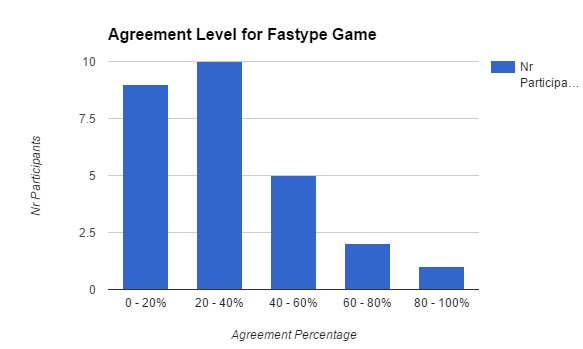
\includegraphics[width=\linewidth]{figures/experiment2/ex2-agreementlevel.PNG}
    \caption{Participant's Agreement Level for Experiment 2}
    \label{fig:game-agreement-level}
\end{figure}

\subsection{Game Design Analysis}
In the previous sub-sections we reported on the performances of non-expert human annotators in terms of annotation quality and agreement level and saw that the quality of annotations did not experience any decrease. In this subsection we report on the performance of Fastype in terms of playfulness, player engagement and see if the players were intrinsically motivated to participate and play the game. 

One of the metrics used to assess the playfulness or the attractiveness of both interfaces (AnnotateMe and Fastype) was by measuring the number of the so-called \textit{free-will annotations}. When conducting each experiment, the participants were instructed to perform their tasks continuously until instructed to stop. An annotation was considered to be a \textit{free-will annotation} when participants free-willingly decided to continue performing tasks even after the experimenter informed them that they have already completed the number of obligatory annotations and were allowed to finish the experiment. Table \ref{tab:free-will-annotation-res} shows the results of free-will annotations performed in both experiments in addition to the average number of tasks performed in a session. The game exhibits a slight improvement over the plain interface in terms of free-will annotations, however, the calculation of one-way Anova resulted in statistically insignificant difference for p = 0.05. The reason for the insignificant difference can be explained by observing the second row of the table, namely, the average annotations performed during an experiment session. We observe that participants performed 50\% more annotations using the plain interface as opposed to the game. Besides the fact that the difference was not significant, we argue that an average of 23\% free-will annotations over an average of 10 game rounds performed by a single participants is better than an average of 17\% free-will annotations over an average of 22 annotation rounds. In a long run, we are confident that the game would perform significantly better and have a significant higher attractiveness as compared to the plain interface. The results presented in Figure \ref{fig:participants-perference} easily back up this claim. 

% Table generated by Excel2LaTeX from sheet 'Sheet6'
\begin{table}[htbp]
  \centering
  \caption{Results of free-will annotations for experiment 1 and 2}
    \begin{tabular}{|l|r|r|}
    \toprule
    \multicolumn{3}{|c|}{\textbf{Participant Average Freewill and total annotations performed}} \\
    \midrule
          & \multicolumn{1}{l|}{\textbf{Fastype Game}} & \multicolumn{1}{l|}{\textbf{AnnotateMe Interface}} \\
    \midrule
    \textbf{Average of free-will annotations} & 23\%    & 17\% \\
    \midrule
    \textbf{Average annotations performed} & 10    & 22 \\
    \bottomrule
    \end{tabular}%
  \label{tab:free-will-annotation-res}%
\end{table}%


\begin{figure}[]
    \centering
    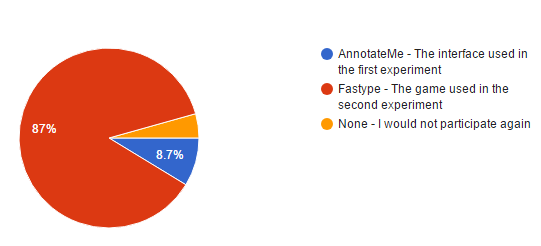
\includegraphics[width=\linewidth]{figures/experiment2/participant-preferance.PNG}
    \caption{Participant's preferred interface for performing annotations}
    \label{fig:participants-perference}
\end{figure}

After both experiments were conducted, we asked participants that took part in both experiments to fill-in a final questionnaire regarding their preferred interface in case they would be asked to do a third experiment. As seen from Figure \ref{fig:participants-perference}, the majority of participants preferred the game compared to AnnotateMe Interface. Please note that the participants had the possibility to choose a third option which allowed participants to express feelings of neutrality or dislike for both interfaces. The third option was provided as a measure against potential bias in our results by allowing all participants who disliked both experience to freely express it. The questionnaire was completely anonymous and was sent through emails where participants completed it from home.

%Post Questionnaire
A post-questionnaire assessing the overall design of the game was also used in the second experiment. In the post-questionnaire, participants were asked different type of questions with each contributing to the assessment of different aspects of game design. Additionally, in order to compare the attractiveness and engagement of participants with the game and the plain interface, both designs were assessed using similar questions in both post-questionnaires. 

%Anova analysis towards experience with interfaces
In order to assess the attractiveness of each interface we asked participants to rate their experience with each interface. The results of the first experiment are shown in the top-right graph presented in Figure \ref{fig:ex1-postresults} whereas the results of the second experiment are presented in Figure \ref{fig:game-experience}. To make sure that the game was perceived as significantly more attractive and fun to use as compared to the plain interface, we run one-way Anova analysis and the results confirm that the difference is statistically significant for p = 0.05 and for p = 0.01. This indicates that the game was perceived significantly more attractive as opposed to the plain interface.

\begin{figure}[]
    \centering
    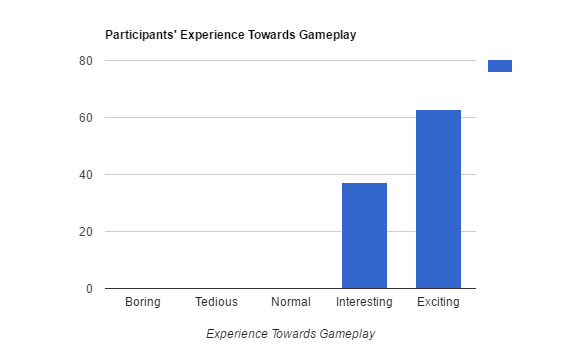
\includegraphics[width=\linewidth]{figures/experiment2/game-participant-experience.PNG}
    \caption{Participant's experience towards the gameplay}
    \label{fig:game-experience}
\end{figure}

%anova analysis about egagement frequency
Regarding the user's perceived engagement with both interfaces, we asked participants how often they would use each interface outside the experiment. Please note that for the same question we unfortunately used different type of answers, with the answer for the first experiment being labels ranging from "Definitely Not" to "Definitely", and the answer for the second experiment being a 7-point liker scale ranging from "Never Again" to "A Lot". However, when calculating one-way Anova, we normalized the 7-point liker scale to 5-point liker scale (dividing the value with 7 and than multiplying it with 5) to be able to properly compare the two observations together (See Appendix \ref{appendix3:engagement_analysis}). The results of the one-way Anova report a statistically significant difference between the two observation for p = 0.05 as well as p = 0.05. These results indicate that the game was perceived as significantly more engaging than the plain interface.  


\begin{figure}[]
    \centering
    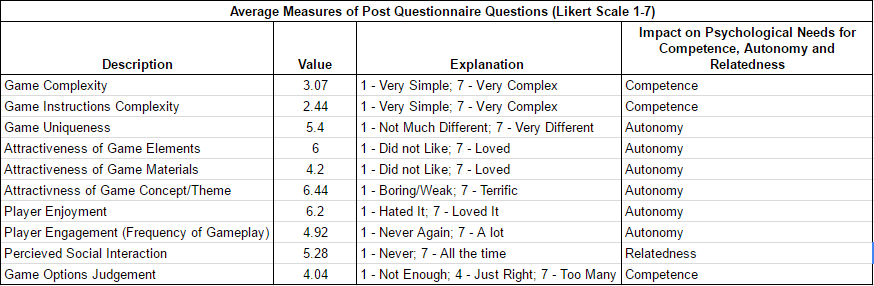
\includegraphics[width=\linewidth]{figures/experiment2/post-questionnaire-final.PNG}
    \caption{Results from the post-questionnaire analysis for experiment 2}
    \label{fig:post-questionnaire-final}
\end{figure}

Finally, Figure \ref{fig:post-questionnaire-final} presents a table with the final results for the rest of the questions used to assess the design of the game on the post-questionnaire. It can be observed that the game scores relatively well in all of the design questions presented to the participants. The table also illustrates the impact of the different game design elements on basic psychological needs for autonomy, competence and relatedness which represent the main factors for affecting player's intrinsic motivation. Since the players perceived the game as generally enjoyable, engaging, socially intractable, easy to adapt with the instruction and rules of the game, genuinely liked the elements, materials and the theme of the game, we claim that the participants were intrinsically motivated to play and do not rely in any other incentive but the desire to be entertained. Consequently, based on these acquired results the first hypothesis of the second experiment is supported (H2.1). The second hypothesis (H2.2) is also supported since the one-way Anova analysis indicate that the participants preferred to use the game significantly more than using the plain interface.  